\documentclass{beamer}
\usetheme{Hannover}
\setbeamersize{sidebar width left=0pt}
\usepackage[T1, T2A]{fontenc}
\usepackage[utf8]{inputenc}
\usepackage[russian]{babel}
\usepackage{hyperref}
\usepackage{graphicx}
\graphicspath{ {../Images/} }

\author{Григорий Матюхин}
\date{\today}
\title{Лабораторная работа \textnumero14.}
\subtitle{Партиции, файловые системы, монтирование}

\begin{document}
\begin{frame}[plain]
	\titlepage
\end{frame}
\section{Цель работы}
\begin{frame}[plain]
	\frametitle{Цель работы}
	Получить навыки создания разделов на диске и файловых систем. Получить навыки монтирования файловых систем.
\end{frame}

\subsection{Создание разделов MBR с помощью \texttt{fdisk}}
\begin{enumerate}
	\begin{frame}[plain]
		\frametitle{Создание разделов MBR с помощью \texttt{fdisk}}
		\item В командной строке с полномочиями администратора с помощью \texttt{fdisk} посмотрите перечень разделов на всех имеющихся в системе устройствах жёстких дисков:
		\\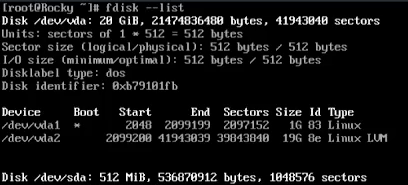
\includegraphics{1.png}
	\end{frame}
	\begin{frame}[plain]
		\item Предположим, что необходимо сделать разметку диска \texttt{/dev/sdb} с помощью утилиты \texttt{fdisk}:
		\\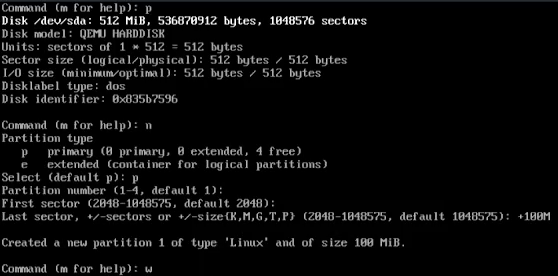
\includegraphics{2.png}
	\end{frame}
\end{enumerate}

\begin{frame}[plain]
	\frametitle{Создание логических разделов}
	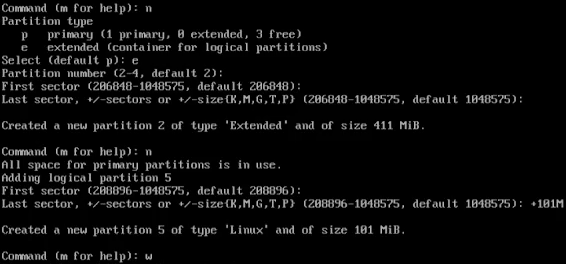
\includegraphics{3.png}
\end{frame}

\begin{frame}[plain]
	\frametitle{Создание раздела подкачки}
	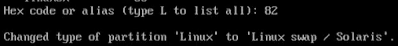
\includegraphics{4.png}
	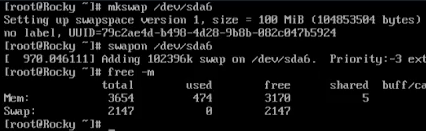
\includegraphics{5.png}
\end{frame}

\begin{frame}[plain]
	\frametitle{Создание разделов GPT с помощью \texttt{gdisk}}
	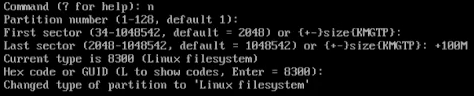
\includegraphics{6.png}
\end{frame}

\begin{frame}[plain]
	\frametitle{Форматирование файловой системы XFS}
	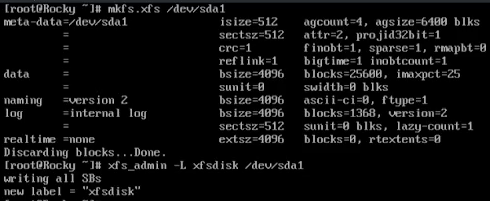
\includegraphics{7.png}
\end{frame}


\begin{frame}[plain]
	\frametitle{Форматирование файловой системы EXT4}
	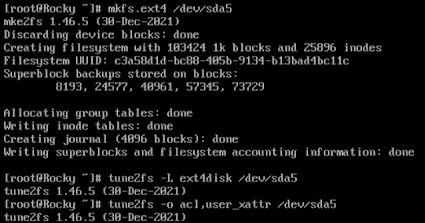
\includegraphics{8.png}
\end{frame}


\begin{frame}[plain]
	\frametitle{Ручное монтирование файловых систем}
	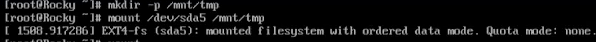
\includegraphics{9.png}
	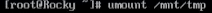
\includegraphics{10.png}
\end{frame}


\begin{frame}[plain]
	\frametitle{Монтирование разделов с помощью \texttt{/etc/fstab}}
	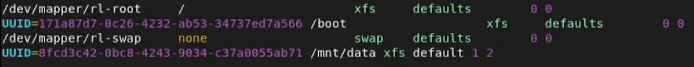
\includegraphics{11.png}
\end{frame}
\begin{frame}[plain]
	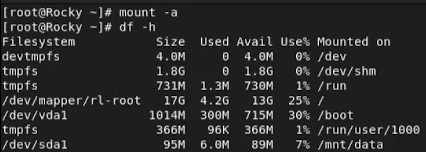
\includegraphics{12.png}
\end{frame}


\begin{enumerate}
	\begin{frame}[plain]
		\frametitle{Самостоятельная работа}
		\item Добавьте две партиции на диск с разбиением GPT.
		Создайте оба раздела размером 100 MiB.
		Один из этих разделов должен быть настроен как пространство подкачки, другой раздел должен быть отформатирован файловой системой ext4.
		\\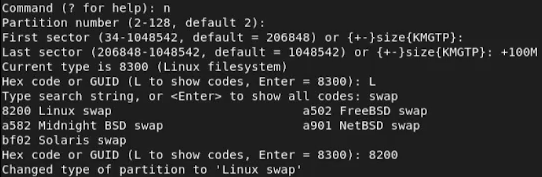
\includegraphics{13.png}
	\end{frame}
	\begin{frame}[plain]
		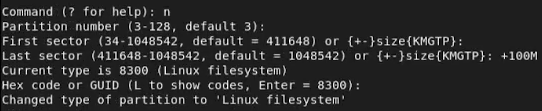
\includegraphics{14.png}
	\end{frame}
	\begin{frame}[plain]

		\item Настройте сервер для автоматического монтирования этих разделов.
		Установите раздел ext4 на \texttt{/mnt/data-ext} и установите пространство подкачки в качестве области подкачки.
		\\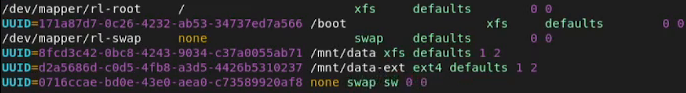
\includegraphics{15.png}
	\end{frame}
	\begin{frame}[plain]
		\item Перезагрузите вашу систему и убедитесь, что всё установлено правильно.
		\\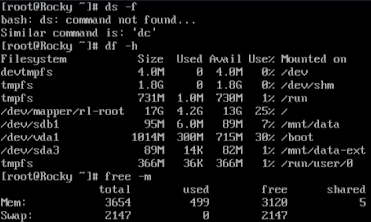
\includegraphics{16.png}
	\end{frame}
\end{enumerate}

\section{Вывод}
\begin{frame}[plain]
	\frametitle{Вывод}
	В ходе выполнения данной работы я получил навыки создания разделов на диске и файловых систем и навыки монтирования файловых систем.
\end{frame}

\end{document}
